\chapter{Intrabundle - An OSGi Bundle Introspection Tool}

\section{Implementation Overview}

\section{Collecting Bundle Data}

\section{Metrics Calculation}

\section{Intrabundle Quality}
In this section we will see how intrabundle quality is managed and how some concepts of \textit{chapter 2 - State of art} were applied to the project.
\subsection{Internal quality}
Intrabundle internal is managed by PMD and Jacoco. PMD is an static analysis tool and JaCoo a dynamic analysis one. Both were presented at Chapter two in section \textit{Quality Analysis Tools} with the objective to guarantee non functional requirements.

\subsubsection{Example}
 A PMD example was already illustrated at Chapter 2 as an example of static analysis tool. JaCoCo is used to calculate code coverage to track files and methods automated tests are covering. Figure 3.1 shows JaCoCo code coverage report for Intrabundle:

\begin{figure}[h]
\caption{Intrabundle code coverage}
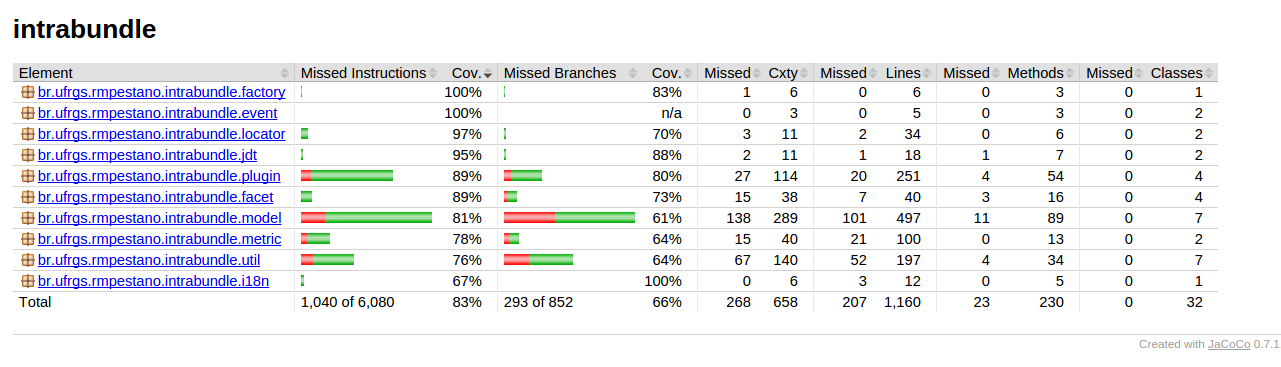
\includegraphics[scale=0.5]{intrabundle-code-coverage}
\end{figure}

\FloatBarrier

\subsection{External quality}
Intrabunde external quality is assured by automated whitebox tests so we can verify if Intrabundle is working as expected, if it meets its functional requirements.

\subsubsection{Example}




